\chapter{神经可塑性、学习与记忆}\label{ch:b3:learning-memory}

1953 年，一位外科医生切除了一名青年患者双侧颞叶的
内侧部分。该患者患有难治性癫痫，发作得以缓解，他
此后五十年间以 H.M. 之名为人所知，再也无法形成关于
事件的持久记忆。他能够交谈，学会在镜子中描摹星形，
与常人一样熟练——但每天都否认自己见过这项任务——
但他仍记得自己的童年。事实表明，记忆并非
单一之物，而新事件记忆的形成则依赖于一个
大小如拇指的结构。大脑学习时发生了什么变化，
是神经科学最古老的问题，其答案来自对一只拥有两万个神经元的
海蛞蝓以及大鼠\omterm{def:b3:learning-memory:kinds}{海马}切片的研究：突触的强度会根据通过它们的
信号而改变，这一规则由唐纳德·赫布于 1949 年推测，
后由一种分子——NMDA 受体——予以实现。
本章讨论该规则及其作用机制，
利用它存储位置与事件的回路，
说明此类系统能学习什么、
能容纳多少的数学理论，
以及告诉它哪些内容值得学习的奖励信号。

\section{记忆的类型及其所在位置}

\begin{definition}[学习与记忆的形式]\label{def:b3:learning-memory:kinds}
\index{习惯化}\index{敏感化}\index{条件反射}\index{陈述性记忆}\index{程序性记忆}\index{巩固}\index{海马}
最简单的学习是\emph{非联合型}的，包括\emph{习惯化}，
对重复出现的无害刺激的反应逐渐减弱，以及
\emph{敏感化}，即受到有害刺激后的反应增强。
\emph{联合型}学习将两个事件联系起来：在\emph{经典
条件反射}（巴甫洛夫）中，预示奖励或惩罚的中性刺激
逐渐引发该反应；在\emph{操作性
条件反射}中，获得奖励的动作会被重复。人类记忆
可分为\emph{陈述性}记忆——即有意识回忆的事实与事件，
依赖于\emph{海马}与内侧颞叶；而\emph{非陈述性}记忆——
即技能与习惯（纹状体、\omterm{def:b3:nervous-systems:plan}{小脑}）、条件性恐惧（杏仁核）、
启动效应（皮层）等，
——以表现形式体现，无需回忆。一段记忆最初
以活性的短时形式保存，持续数秒至数小时，并
在数小时至数年内被\emph{巩固}为稳定的长时形式，
不再依赖海马，而储存于皮层中。
\end{definition}

\begin{proof}[证据]
斯科维尔与米尔纳（1957）报道了 H.M. 的情况：
切除双侧\omterm{def:b3:learning-memory:kinds}{海马}及邻近皮层后，他的智力与手术前的记忆大体完好，
其工作记忆在注意力集中时正常，
但他无法形成任何关于事件或事实的新记忆。
他学习运动技能的速度在数日内与常人相当，
却否认自己曾练习过，因此技能记忆不需要\omterm{def:b3:learning-memory:kinds}{海马}；
他对遥远往事的记忆好于手术前数年的记忆，
因此\omterm{def:b3:learning-memory:kinds}{海马}的作用在于形成\omterm{def:b3:learning-memory:kinds}{陈述性记忆}，
并在一段时间内保持它们，而非永久储存。
具有相同\omterm{def:b3:dna-repair:lesions}{损伤}的猴子与大鼠也表现出同样的分离现象，
而对这一单个患者的研究
重塑了整个领域。
\end{proof}

\section{赫布规则及其分子}

\begin{definition}[赫布可塑性、LTP 与 LTD]\label{def:b3:learning-memory:ltp}
\index{赫布规则}\index{长时程增强}\index{长时程抑制}\index{峰电位时序依赖可塑性}
赫布（1949）提出：当突触前神经元反复参与
使突触后神经元放电时，两者之间的连接得到加强——
“同时放电的细胞会连接在一起”。
\emph{长时程增强}（LTP）是其实验形式：短暂的
高频刺激串作用于某一通路，使被激活的突触
在脑片中维持数小时，在动物体内则维持数周。
LTP 具有\emph{输入特异性}（仅受刺激的突触
改变）、\emph{联合型}（与同一细胞的强输入配对的弱输入
得到增强），并需要输入之间的\emph{\omterm{def:b3:structural-biology:allostery}{协同性}}
才能使细胞去极化。\emph{长时程抑制}（LTD）是其
相反过程，由长时间低频活动引起。在
\emph{峰电位时序依赖可塑性}中，符号由先后顺序决定：一个
突触前峰电位在突触后峰电位\emph{之前}几毫秒，
使突触增强；恰在其\emph{之后}则使突触减弱，
两者均在约 \qty{20}{ms} 的时间窗内发生——因此突触
学会的是预测，而不仅仅是关联。
\end{definition}

\begin{proposition}[作为符合检测器的 NMDA 受体]\label{prop:b3:learning-memory:nmda}
\index{NMDA 受体}\index{AMPA 受体}\index{CaMKII}\index{CREB}\index{树突棘}
在兴奋性突触处，谷氨酸作用于两种受体。其中
\emph{AMPA} 受体在结合后开放，携带普通的
突触电流。\emph{NMDA} 受体可结合谷氨酸，但在静息电位下
被其孔道中的镁离子阻断；只有当
突触后膜去极化——由多个输入同时引起，或
由逆向传播的动作电位引起——镁离子才被排出，
通道开放，允许钙离子内流。因此 NMDA 受体
仅在突触前释放（谷氨酸）与突触后活动
（去极化）同时出现时才开放：它是赫布所说的“与”门，
集于一个蛋白质之中。进入\emph{\omterm{prop:b3:learning-memory:nmda}{树突棘}}的钙离子
激活激酶\emph{\omterm{prop:b3:learning-memory:nmda}{CaMKII}}，后者使 AMPA 受体磷酸化，
并将更多受体从储备中转入突触——突触
在数分钟内即增强（早期 LTP）。缓慢而大幅的钙离子升高
则激活磷酸酶钙调神经磷酸酶，后者移除
AMPA 受体，产生 LTD。持续数小时以上的增强（晚期 LTP）
需要新合成的蛋白质：激酶进入细胞核，转录因子
\emph{\omterm{prop:b3:learning-memory:nmda}{CREB}} 开启基因，\omterm{prop:b3:learning-memory:nmda}{树突棘}生长，甚至可能分裂——
这与在所研究的每种动物中区分短时与
长时记忆的基因表达要求相同。
\end{proposition}

\begin{proof}[证据]
布利斯与勒莫（1973）以脉冲串刺激通往兔\omterm{def:b3:learning-memory:kinds}{海马}的
穿通通路，发现诱发反应在随后数小时内明显增大，此即首次
观察到的 LTP。科林格里奇（1983）证明，\omterm{prop:b3:learning-memory:nmda}{NMDA
受体}阻断剂（AP5）能阻止 LTP 的诱导，却不影响
普通突触反应；莫里斯（1986）将 AP5 注入大鼠\omterm{def:b3:learning-memory:kinds}{海马}，
发现大鼠在水池中游泳并能正常视物时，已无法
学会隐藏平台的位置；而在 \omterm{def:b3:learning-memory:hippocampus}{CA1} 区单独缺失
NMDA 受体的小鼠，该区既缺失 LTP，也缺失
空间记忆。同一受体，位于同一位置，既是突触变化
的必要条件，
也是学习的必要条件。
\end{proof}

\begin{omfigure}
\begin{tikzpicture}[every node/.style={font=\scriptsize}, >=stealth]
  % presynaptic terminal
  \draw[thick, omDef, fill=omDef!12] (0,2.2) .. controls (0,3.4) and (4,3.4) .. (4,2.2) -- (4,1.7) -- (0,1.7) -- cycle;
  \node at (2,2.8) {突触前末梢};
  \foreach \p in {(0.8,2.0),(1.6,2.1),(2.6,2.0),(3.3,2.1)} \draw[thick, fill=omDef!40] \p circle (0.17);
  \foreach \p in {(1.2,1.45),(2.0,1.5),(2.9,1.42)} \fill[omProp] \p circle (0.06);
  \node[right, omProp] at (3.3,1.45) {谷氨酸};
  % postsynaptic spine
  \draw[thick, omMeth!70!black, fill=omMeth!10] (-0.6,1.1) -- (4.4,1.1) -- (4.4,-1.2) -- (-0.6,-1.2) -- cycle;
  \node at (0.6,-0.9) {树突棘};
  % AMPA
  \draw[thick, fill=omMeth!45] (0.2,0.85) rectangle (0.6,1.35); \node[below, align=center] at (0.1,0.8) {AMPA:\\Na$^{+}$ 内流};
  \draw[->, thick] (0.4,1.7) -- (0.4,0.95);
  % NMDA with Mg
  \draw[thick, fill=omThm!35] (2.4,0.85) rectangle (2.9,1.35); \fill[gray!70] (2.65,1.1) circle (0.09); \node[right, font=\tiny] at (2.95,1.1) {Mg$^{2+}$ 阻断};
  \node[below, align=center] at (2.65,0.8) {NMDA：需要谷氨酸 \\\emph{且}去极化};
  \draw[->, thick, omThm] (2.65,0.15) -- (2.65,-0.5) node[below] {Ca$^{2+}$};
  % downstream
  \node[draw, rounded corners, fill=omThm!15, font=\tiny] (cam) at (5.6,0.3) {CaMKII 激酶};
  \draw[->, thick] (2.9,-0.5) -- (cam);
  \node[draw, rounded corners, fill=omMeth!25, font=\tiny, align=center] (ampa) at (8.2,1.0) {AMPA 受体插入增多 \\早期 LTP（数分钟）};
  \node[draw, rounded corners, fill=omMeth!25, font=\tiny, align=center] (creb) at (8.2,-0.5) {CREB、新蛋白质、\\棘生长：晚期 LTP（数小时以上）};
  \draw[->, thick] (cam) -- (ampa.west); \draw[->, thick] (cam) -- (creb.west);
  \node[draw, rounded corners, fill=omDef!15, font=\tiny, align=center] (ltd) at (8.2,-1.8) {慢而少的 Ca$^{2+}$：钙调神经磷酸酶，\\AMPA 移除：LTD};
  \draw[->, thick, dashed] (2.9,-0.7) .. controls (4.5,-1.6) .. (ltd.west);
\end{tikzpicture}

{\small NMDA 受体作为赫布的“门”。仅有谷氨酸即可打开 \omterm{prop:b3:learning-memory:nmda}{AMPA
受体}；只有当棘同时去极化、镁离子移开后，NMDA 通道才导通。
随之内流的钙决定了突触的未来：快速而大量的钙升高使其增强，
缓慢而少量的钙升高
则使其减弱。}
\end{omfigure}

\begin{omfigure}
\begin{tikzpicture}
\begin{axis}[
  width=6.6cm, height=5.2cm,
  axis x line=bottom, axis y line=left,
  xmin=-20, xmax=120, ymin=0, ymax=220,
  xlabel={分钟}, ylabel={突触反应（\%）},
  xlabel style={font=\small, at={(axis description cs:0.5,-0.12)}, anchor=north}, ylabel style={font=\small},
  tick label style={font=\scriptsize}, xtick={0,30,60,90,120}, ytick={0,100,200},
  clip=false,
]
\addplot[only marks, mark=*, mark size=1pt, omDef] coordinates {(-18,100) (-15,98) (-12,102) (-9,99) (-6,101) (-3,100) (2,195) (5,180) (8,172) (11,168) (15,165) (20,162) (30,160) (40,158) (50,157) (60,156) (70,156) (80,155) (90,155) (100,154) (110,154) (120,154)};
\addplot[only marks, mark=o, mark size=1pt, gray] coordinates {(-18,100) (-12,101) (-6,99) (2,102) (8,100) (15,101) (30,100) (45,99) (60,101) (75,100) (90,100) (105,101) (120,100)};
\draw[->, thick, omThm] (axis cs:0,215) -- (axis cs:0,200); \node[font=\scriptsize, omThm, anchor=south] at (axis cs:0,216) {强直收缩};
\node[font=\scriptsize, omDef, anchor=south west] at (axis cs:35,168) {受刺激通路：LTP};
\node[font=\scriptsize, gray, anchor=north west] at (axis cs:35,95) {对照通路：无变化};
\end{axis}
\begin{axis}[
  at={(7.6cm,0)}, anchor=south west,
  width=6.6cm, height=5.2cm,
  axis x line=middle, axis y line=middle,
  xmin=-60, xmax=60, ymin=-60, ymax=100,
  xlabel={$t_{\text{突触前}} - t_{\text{突触后}}$ (ms)}, ylabel={$\Delta w$ (\%)},
  xlabel style={font=\small,  at={(axis description cs:0.5,-0.06)}, anchor=north}, ylabel style={font=\small, at={(axis description cs:0.5,1.02)}, anchor=south},
  tick label style={font=\scriptsize}, xtick={-40,-20,20,40}, ytick={-40,40,80},
  clip=false,
]
\addplot[very thick, omMeth!70!black, domain=-60:-0.5, samples=60] {80*exp(x/15)};
\addplot[very thick, omThm, domain=0.5:60, samples=60] {-45*exp(-x/25)};
\node[font=\scriptsize, omMeth!70!black, anchor=south east] at (axis cs:-8,62) {突触前先于突触后：LTP};
\node[font=\scriptsize, omThm, anchor=north west] at (axis cs:8,-22) {突触后先于突触前：LTD};
\end{axis}
\end{tikzpicture}

{\small 左：\omterm{def:b3:learning-memory:ltp}{长时程增强}——短暂强直刺激后，受刺激通路的
反应持续数小时增大，而接到同一细胞的未受刺激通路
保持不变（输入特异性）。右：峰电位时序窗——若突触前峰电位
先于突触后，突触增强；若滞后，
则突触减弱。}
\end{omfigure}

\begin{theorem}[赫布突触学到什么]\label{thm:b3:learning-memory:hebb}
\index{赫布学习!主成分}\index{Oja 规则}
设神经元接收输入 $\mathbf{x} = (x_{1},\dots,x_{n})$，
经权重 $\mathbf{w}$ 作线性响应，$y = \mathbf{w}\cdot\mathbf{x}$。
\omterm{def:b3:learning-memory:ltp}{赫布规则} $\Delta\mathbf{w} = \eta\, y\,\mathbf{x}$，
对输入取平均后给出
\[
\langle\Delta\mathbf{w}\rangle = \eta\,C\,\mathbf{w}, \qquad C =
\langle\mathbf{x}\mathbf{x}^{\mathsf{T}}\rangle ,
\]
其中 $C$ 为输入的相关矩阵。权重
无界增长，且沿 $C$ 的
最大本征值所对应的特征向量增长最快：突触逐渐识别出最常出现的输入模式
——即其输入的\emph{主成分}。
若加入惩罚大权重的项，得到\emph{Oja 规则}
$\Delta\mathbf{w} = \eta\, y\,(\mathbf{x} - y\,\mathbf{w})$，权重向量
收敛到该特征向量并归一化为单位长度，神经元
成为对所见输入中主导相关性的稳定
检测器。
\end{theorem}
\begin{proof}
将 $y = \mathbf{w}\cdot\mathbf{x} = \mathbf{x}^{\mathsf{T}}
\mathbf{w}$ 代入\omterm{def:b3:learning-memory:ltp}{赫布规则}，得 $\Delta\mathbf{w} = \eta\,\mathbf{x}
\mathbf{x}^{\mathsf{T}}\mathbf{w}$，其对输入的平均（设
$\mathbf{w}$ 变化缓慢）为 $\eta C\mathbf{w}$。$C$ 对称且
半正定，故有正交特征向量 $\mathbf{e}_{k}$，
对应本征值 $\lambda_{k} \ge 0$；记 $\mathbf{w} = \sum_{k}
a_{k}\mathbf{e}_{k}$，各分量满足 $\Delta a_{k} = \eta\lambda_{k}
a_{k}$，并按 $(1 + \eta\lambda_{k})^{t}$ 增长，因此沿
最大本征值方向的分量将主导 $\mathbf{w}$ 的方向，
同时其长度\omterm{def:b3:nervous-systems:circuits}{发散}。Oja 规则取平均后为 $\eta(C\mathbf{w} -
(\mathbf{w}^{\mathsf{T}}C\mathbf{w})\mathbf{w})$；在不动点处
$C\mathbf{w} = (\mathbf{w}^{\mathsf{T}}C\mathbf{w})\mathbf{w}$，故
$\mathbf{w}$ 为特征向量，且 $\lambda = \mathbf{w}^{\mathsf{T}}
C\mathbf{w} = \lambda|\mathbf{w}|^{2}$，因而 $|\mathbf{w}| = 1$；
沿最大本征值的不动点是稳定的（
向另一特征向量的微扰会衰减，因为该特征向量
的本征值更小），此处在本阶段不加证明地承认。
\end{proof}

\begin{example}[两个输入]\label{ex:b3:learning-memory:two-inputs}
一个神经元接收两个通常同时活跃的输入，因此 $C =
\begin{pmatrix} 1 & 0.8 \\ 0.8 & 1\end{pmatrix}$。其特征向量为
$(1,1)/\sqrt{2}$ 对应本征值 $1.8$，$(1,-1)/\sqrt{2}$ 对应
本征值 $0.2$。从 $\mathbf{w} = (1, 0)$ 出发，\omterm{def:b3:learning-memory:ltp}{赫布规则}经过许多小步更新后，
$\mathbf{w}$ 转向 $(1,1)$：神经元学会
对两个输入\emph{同时}作出响应，并忽略少见的
只有一个输入放电的情形——它提取出了相关性。
采用奥亚规则时，权重稳定在 $(0.71, 0.71)$。这正是
赫布式突触学会“哪些事物总是一同出现”的含义，也
解释了\omterm{def:b3:learning-memory:ltp}{长时程增强}的联合性，即把弱输入与强输入配对，
可由该规则推出。
\end{example}

\section{会学习的海蛞蝓}

\begin{proposition}[\emph{Aplysia} 中的敏感化]\label{prop:b3:learning-memory:aplysia}
\index{Aplysia}\index{突触前易化}\index{cAMP}\index{PKA}
海蛞蝓 \emph{\omterm{prop:b3:learning-memory:aplysia}{Aplysia}} 在水管受到触碰时会缩回其
鳃，这是一种由几十个可辨认神经元构成的反射。尾部受
到电击后会使其\emph{\omterm{def:b3:learning-memory:kinds}{敏感化}}：对轻触的缩回反应增强，
单次电击后持续数分钟，多次电击后持续数周。坎德尔与同事
（1970 年代至 1990 年代）追踪到这一变化发生在水管感觉神经元与鳃运动神经元之间的
突触上。尾部电击兴奋一个\omterm{def:b3:nervous-systems:cells}{中间神经元}，
该神经元向感觉神经元的末端释放 5-羟色胺；
5-羟色胺提高环 AMP 水平，环 AMP 激活
蛋白激酶 A，它使一个钾通道磷酸化并使其关闭；
末端的动作电位展宽，钙离子内流增加，每次
放电释放的递质增多——\emph{\omterm{prop:b3:learning-memory:aplysia}{突触前易化}}，
这是一种持续数分钟的共价修饰。重复电击使该激酶
进入细胞核，在那里激活 \omterm{prop:b3:learning-memory:nmda}{CREB}，后者开启
能够构建新突触末端的基因：长时记忆即突触数量的增加，
训练期间给予蛋白质合成抑制剂会阻断它，
训练结束后给予则无效。\emph{\omterm{def:b3:learning-memory:kinds}{习惯化}}恰好相反，
即同一突触上的一种抑制；而\emph{经典\omterm{def:b3:learning-memory:kinds}{条件反射}}，
即把触碰与电击配对，增强
在五羟色胺到达前恰好活跃的突触上的易化——
一种以突触前方式实现的赫布式巧合，由
同时受钙离子与五羟色胺刺激的腺苷酸环化酶完成。
\end{proposition}

\begin{omfigure}
\begin{tikzpicture}[every node/.style={font=\scriptsize}, >=stealth]
  \node[draw, thick, rounded corners, fill=omDef!20, minimum width=2cm] (sn) at (0,0) {水管感觉神经元};
  \node[draw, thick, rounded corners, fill=omMeth!25, minimum width=2cm] (mn) at (6.2,0) {鳃运动神经元};
  \node[draw, thick, rounded corners, fill=omProp!30, align=center] (in) at (2.8,2.4) {易化性中间神经元 \\（五羟色胺）};
  \node[left] at (-2.1,0) {触碰}; \draw[->, thick] (-2.0,0) -- (sn);
  \draw[->, very thick] (sn) -- (mn) node[pos=0.45, below, align=center, font=\tiny] {发生变化的 \\突触};
  \draw[->, thick] (mn) -- (8.4,0) node[right] {鳃缩回};
  \node[above] at (2.8,3.1) {尾部电击}; \draw[->, thick] (2.8,3.05) -- (in);
  \draw[->, thick, omProp] (in) -- (2.8,0.25);
  \node[right, align=left, font=\tiny] at (6.6,1.6) {5-羟色胺 $\to$ cAMP $\to$ PKA $\to$ K$^{+}$ 通道关闭 \\$\to$ 动作电位展宽，Ca$^{2+}$ 增多，递质增多（数分钟）\\重复时：PKA $\to$ CREB $\to$ 新末端（数周）};
\end{tikzpicture}

{\small \emph{\omterm{prop:b3:learning-memory:aplysia}{Aplysia}} 的\omterm{def:b3:learning-memory:kinds}{敏感化}回路。来自一个
\omterm{def:b3:nervous-systems:cells}{中间神经元}的 5-羟色胺作用于感觉末端，同一突触
以磷酸化通道的形式承载短时记忆，并以新末端的形式
承载长时记忆。}
\end{omfigure}

\begin{omfigure}
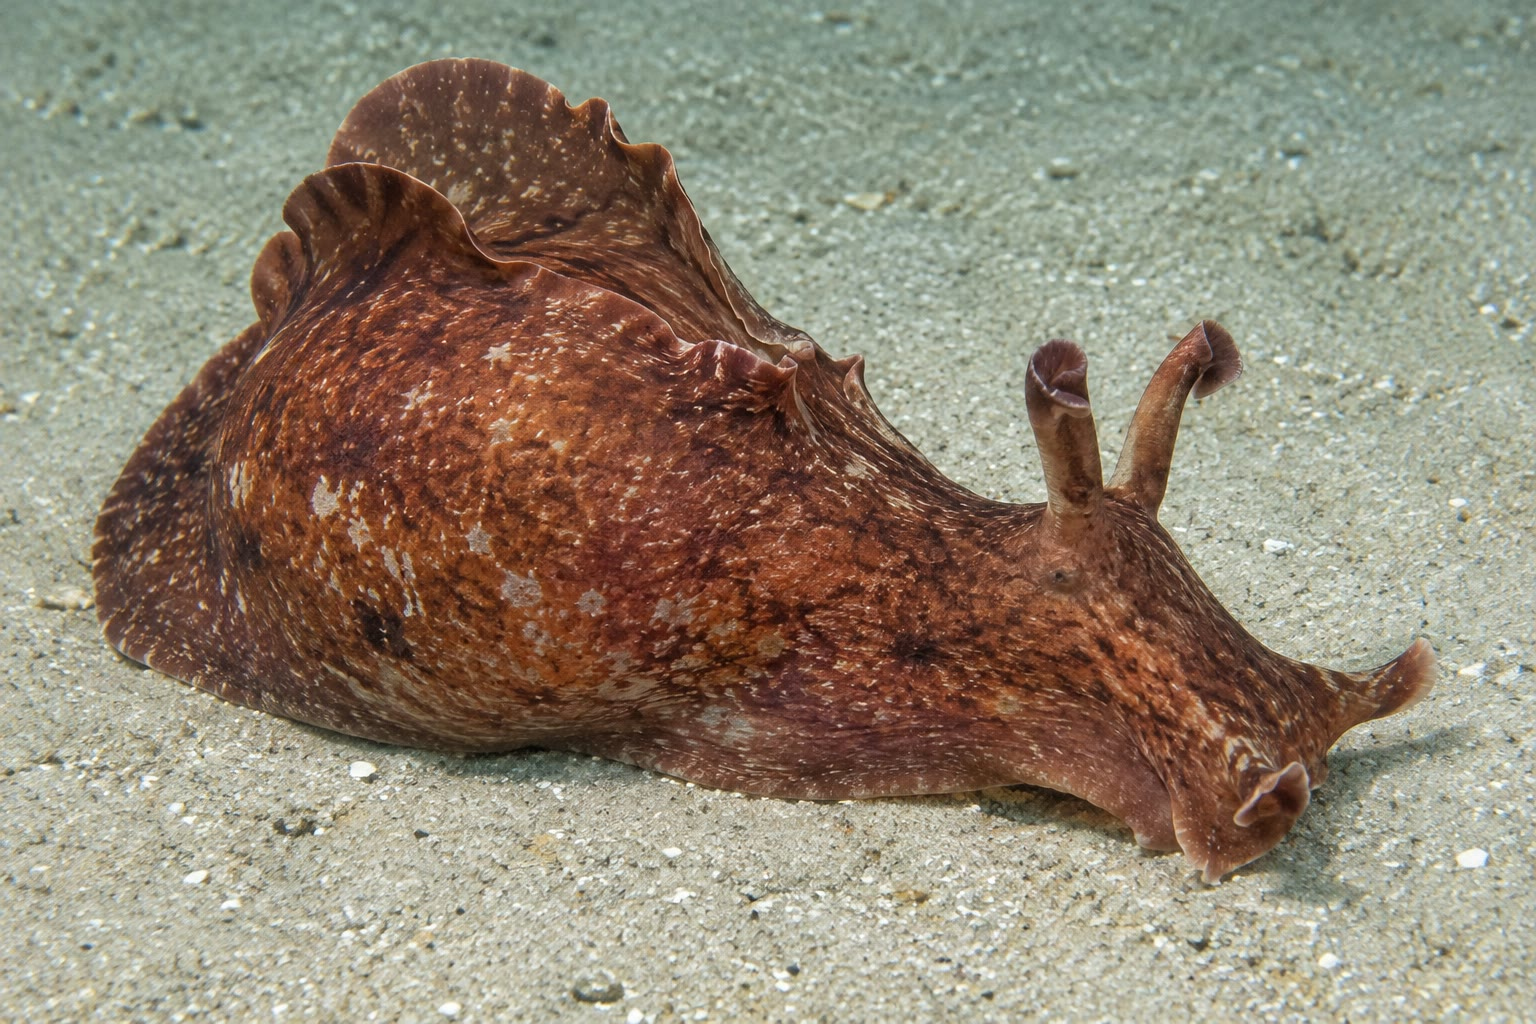
\includegraphics[width=0.46\linewidth]{images/book5/ai/b5-19-aplysia.jpg}\hspace{0.04\linewidth}
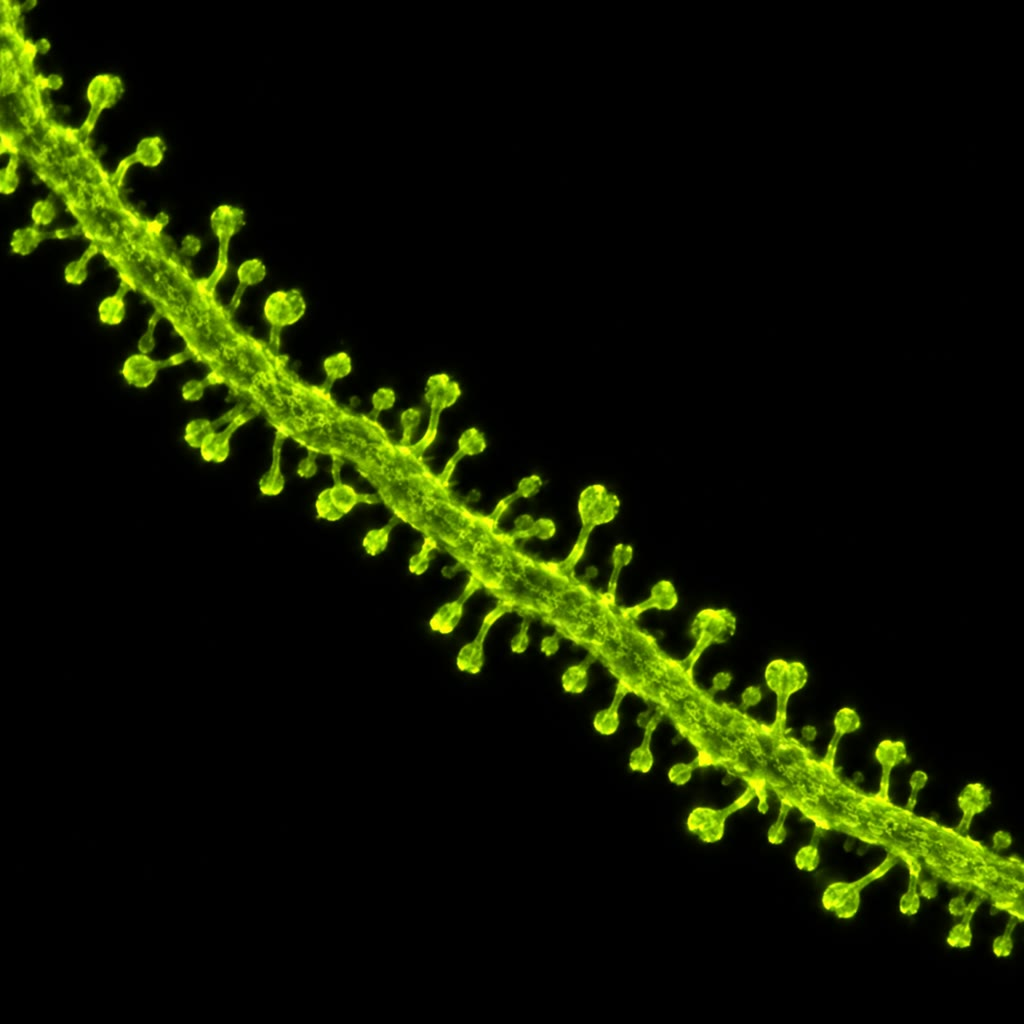
\includegraphics[width=0.36\linewidth]{images/book5/ai/b5-19-dendritic-spines.jpg}

{\small 左：\emph{\omterm{prop:b3:learning-memory:aplysia}{Aplysia} californica}，其神经元少而大，
使记忆所对应的突触得以被找到并记录。右：一段树突
上布满\omterm{prop:b3:learning-memory:nmda}{树突棘}，每个\omterm{prop:b3:learning-memory:nmda}{树突棘}是一个兴奋性突触的突触后侧，
且各自构成一个区室，其内钙离子决定该棘突自身的命运。}
\end{omfigure}

\section{位置与事件的回路}

\begin{definition}[海马回路]\label{def:b3:learning-memory:hippocampus}
\index{齿状回}\index{CA3}\index{CA1}\index{位置细胞}\index{网格细胞}\index{模式补全}\index{重放}
皮层输入经由内嗅皮层到达\omterm{def:b3:learning-memory:kinds}{海马}，
并依次经过三个阶段：\emph{齿状回}，其
颗粒细胞数目多于其输入，且稀疏放电（分离
相似模式）；\emph{CA3}，其锥体细胞
彼此递归连接，每个细胞接收来自其他细胞的数千个突触
——一个\emph{自联想}网络，能够从片段补全已存储的
模式；\emph{CA1}，它将 CA3 的输出与直接输入进行比较，
并将结果送回皮层。在大鼠
探索场地时，\omterm{def:b3:learning-memory:kinds}{海马}锥体细胞仅在
动物位于某一处时才放电——即一种\emph{位置细胞}（奥基夫，1971）——
数百个这样的细胞即可描绘整个场地；在上游的内嗅皮层中，
\emph{网格细胞}（莫泽，2005）在覆盖空间的六边形
晶格顶点处放电，这是一个坐标系，位置野
由此构建。在睡眠和休息期间，跑步时放电的位置细胞序列
以高速被\emph{重放}，而阻断
重放会损害对该次跑动的记忆：\omterm{def:b3:learning-memory:kinds}{海马}把
当天的路径向皮层反复演练。
\end{definition}

\begin{omfigure}
\begin{tikzpicture}[every node/.style={font=\scriptsize}, >=stealth]
  % trisynaptic loop
  \node[draw, thick, rounded corners, fill=gray!15, align=center] (ec) at (0,0) {内嗅皮层 \\（网格细胞）};
  \node[draw, thick, rounded corners, fill=omDef!20, align=center] (dg) at (3.2,1.4) {齿状回：\\模式分离};
  \node[draw, thick, rounded corners, fill=omProp!30, align=center] (ca3) at (7.2,1.4) {CA3，递归连接：\\模式补全};
  \node[draw, thick, rounded corners, fill=omMeth!25, align=center] (ca1) at (7.2,-1.4) {CA1：\\比较、输出};
  \draw[->, thick] (ec) -- (dg); \draw[->, thick] (dg) -- (ca3); \draw[->, thick] (ca3) -- (ca1); \draw[->, thick] (ca1) -- (ec) node[pos=0.3, below, sloped, font=\tiny] {返回皮层};
  \draw[->, thick, dashed] (ec) -- (ca1.north west) node[pos=0.7, above, sloped, font=\tiny] {直接通路};
  \draw[->, thick, omProp!80!black] (ca3.north) .. controls (6.6,2.6) and (7.8,2.6) .. (ca3.north east) node[pos=0.5, above, font=\tiny] {递归侧支};
  % place field map
  \begin{scope}[xshift=10.4cm, yshift=-0.2cm]
    \draw[thick] (0,0) rectangle (3,2.4); \node[below] at (1.5,-0.05) {从上方所见的场地};
    \foreach \p/\c in {(0.7,1.8)/omThm, (2.1,1.9)/omDef, (1.4,0.9)/omMeth, (2.5,0.6)/omProp} { \fill[\c!60] \p circle (0.32); \fill[\c!90] \p circle (0.16); }
    \node[above] at (1.5,2.45) {四个位置细胞的放电野};
  \end{scope}
\end{tikzpicture}

{\small 左：\omterm{def:b3:learning-memory:kinds}{海马}环路——\omterm{def:b3:learning-memory:hippocampus}{齿状回}中的分离，
存储与补全发生在循环连接的 \omterm{def:b3:learning-memory:hippocampus}{CA3} 区，比较发生在 \omterm{def:b3:learning-memory:hippocampus}{CA1} 区。右：
每个\omterm{def:b3:learning-memory:hippocampus}{位置细胞}在一个场地的某一区域中放电；它们共同绘出
空间。}
\end{omfigure}

\begin{proposition}[自联想网络能容纳多少记忆]\label{prop:b3:learning-memory:capacity}
\index{霍普菲尔德网络}\index{记忆容量}
由 $N$ 个神经元组成的网络，每个神经元与其他所有神经元相连，
连接权重为赫布权重 $w_{ij} \propto \sum_{\mu}\xi_{i}^{\mu}\xi_{j}^{\mu}$，
其中对所存储的二值模式 $\xi^{\mu}$ 求和。该网络能从受损或
不完整的线索中检索出已存储的模式，方法是沉降到该模式对应的
吸引子上（霍普菲尔德，1982）。它在约 $P
\approx 0.14N$ 个随机模式以内时可靠地工作；超过此数，模式之间
发生干涉，检索随之失效。以大鼠的 \omterm{def:b3:learning-memory:hippocampus}{CA3} 区为例，它约有 $3\times 10^{5}$ 个锥体
细胞，按此估算可保有约 $4\times 10^{4}$ 个模式 ---
大致相当于动物在一个季节中所遇到的不同地点或情节的数量级 ---
而其稀疏放电（任一模式中仅有百分之几的细胞活跃）
进一步提高了容量。由线索完成\omterm{def:b3:learning-memory:hippocampus}{模式补全}，
使得一种气味或一个角落便可唤起整个场景；其代价是
相似的记忆相互融合，而\omterm{def:b3:learning-memory:hippocampus}{齿状回}的分离作用对此加以抵抗。
\end{proposition}
\admitted

\begin{method}[记忆及其机制的检验]\label{met:b3:learning-memory:tests}
\index{莫里斯水迷宫}\index{恐惧条件反射}\index{记忆痕迹}
（1）一项空间任务：\omterm{met:b3:learning-memory:tests}{莫里斯水迷宫}——大鼠在不透明的水中游动，
寻找藏于固定位置的平台，并
依据房间内的线索，在数天内学会其位置，并以撤去平台后其在正确象限中的搜寻时间来检验；
\omterm{def:b3:learning-memory:kinds}{海马}\omterm{def:b3:dna-repair:lesions}{损伤}、
NMDA 阻断剂与 LTP 的丧失，各自都会使学习消失。（2）
一项联想任务：\omterm{met:b3:learning-memory:tests}{恐惧条件反射}——将一个音调与足部电击配对，
使其引发僵直；该记忆依赖于杏仁核，而
与情境相关的版本则依赖于\omterm{def:b3:learning-memory:kinds}{海马}。（3）机制检验：
阻断候选机制（如某种药物，或仅限于某一脑区和时段的基因\omterm{def:b3:genetic-engineering:transgenic}{敲除}）
，并证明学习失败，而感知与运动
不受影响。（4）\omterm{met:b3:learning-memory:tests}{记忆痕迹}：标记学习期间活跃的神经元，所用的是
光敏通道（见\cref{ch:b3:nervous-systems}），之后
再用光将其重新激活——动物在安全情境中出现僵直，仿佛
在回忆；抑制它们则阻断回忆。记忆存在于可辨认的
细胞及其突触之中，并可被开启与关闭。
\end{method}

\begin{omfigure}
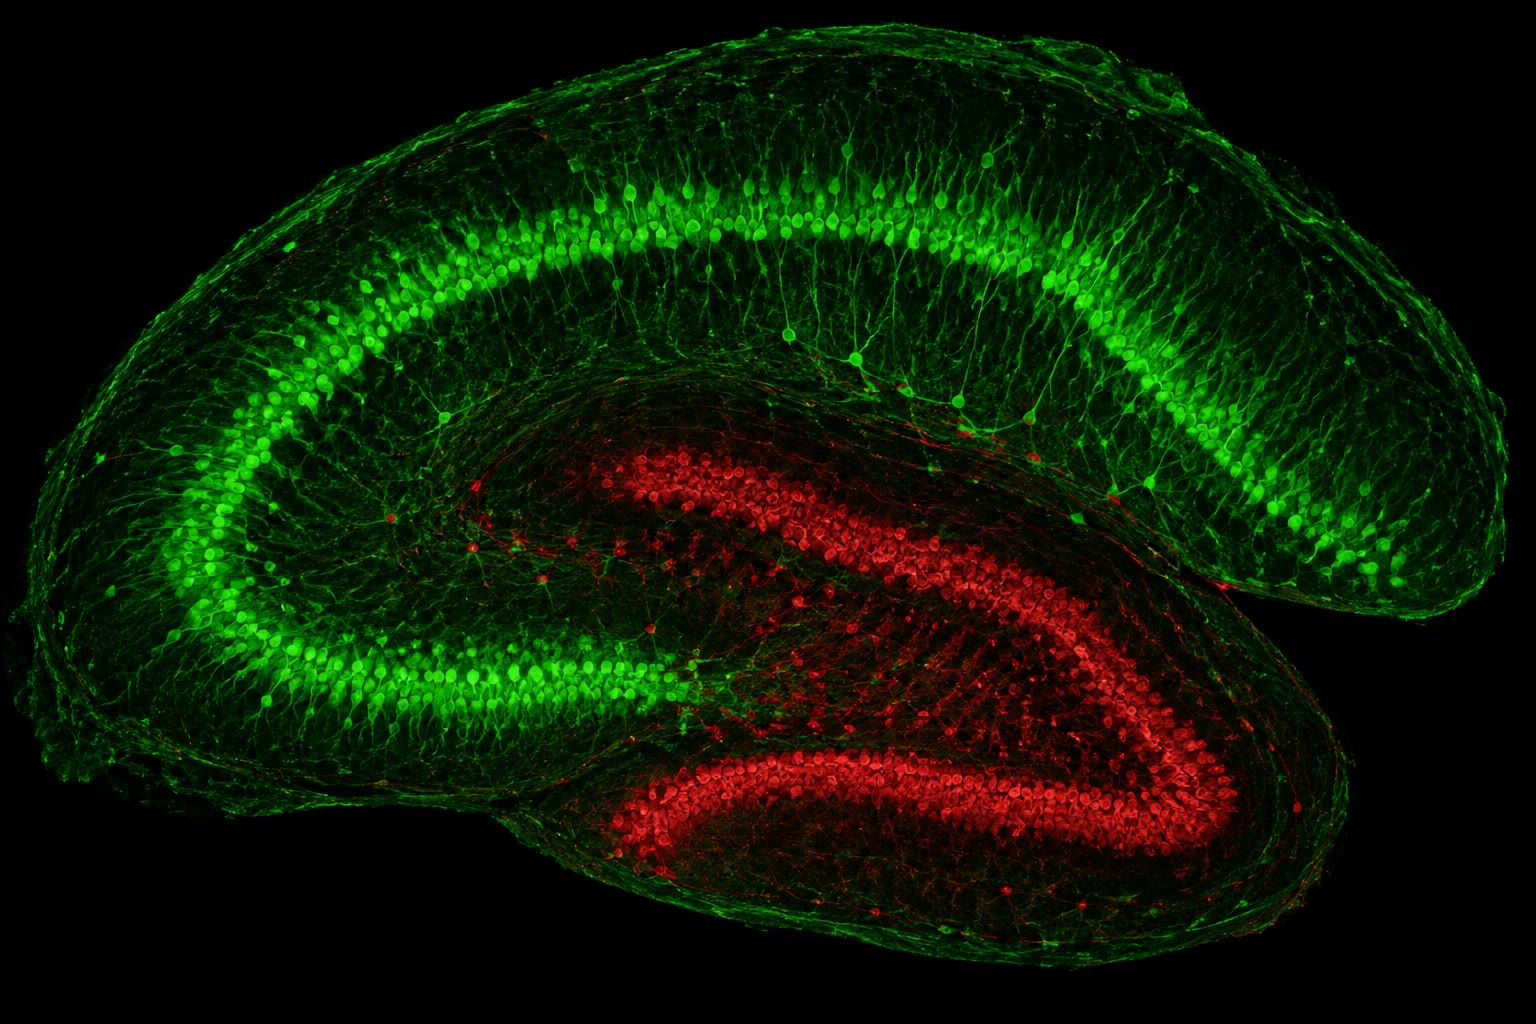
\includegraphics[width=0.56\linewidth]{images/book5/ai/b5-19-hippocampus-section.jpg}

{\small 啮齿类动物\omterm{def:b3:learning-memory:kinds}{海马}切片：自 \omterm{def:b3:learning-memory:hippocampus}{CA3} 至 \omterm{def:b3:learning-memory:hippocampus}{CA1} 的弯曲锥体细胞带
（绿色）以及相互嵌合的\omterm{def:b3:learning-memory:hippocampus}{齿状回}
（红色）。动物的每一项空间记忆都要经过这一
环路。}
\end{omfigure}

\section{奖赏、预测与一生的可塑性}

\begin{proposition}[由预测误差学习]\label{prop:b3:learning-memory:rescorla}
\index{雷斯科拉–瓦格纳规则}\index{预测误差}\index{多巴胺}
设 $V$ 为动物赋予某一线索的价值，$\lambda$ 为
紧随其后的奖赏。\omterm{prop:b3:learning-memory:rescorla}{雷斯科拉–瓦格纳规则}（1972）指出，在
每次试验中，价值的变化量为
$\alpha$ 倍的\emph{\omterm{prop:b3:learning-memory:rescorla}{预测误差}}：
\[
\Delta V = \alpha\,(\lambda - V), \qquad
V_{n} = \lambda\bigl(1 - (1-\alpha)^{n}\bigr) ,
\]
因此学习起初较快，随着预测改善而变慢，
在奖赏被完全预测时停止，并在奖赏被扣留时逆转
（即消退）。当两个线索同时出现时，它们
共享一个预测，因此对于一个对既有预测毫无增益的线索，
则不会被习得（\emph{阻断}）。舒尔茨（1997）记录了
猴子中脑的\omterm{prop:b3:learning-memory:rescorla}{多巴胺}神经元，发现它们
对意外奖赏放电，对完全被预测的奖赏则保持沉默，并在
预期奖赏未能出现时降至基线以下：它们广播
$\lambda - V$，即\omterm{prop:b3:learning-memory:rescorla}{预测误差}本身，传递至纹状体与皮层，
在那里，\omterm{prop:b3:learning-memory:rescorla}{多巴胺}对近期
活跃的突触的可塑性进行门控。学习何种线索预示奖赏，正是带有一个
第三因子的赫布可塑性，该因子说明结果是好于还是差于
预期——而\omterm{def:b3:learning-memory:critical}{成瘾}性药物直接驱动\omterm{prop:b3:learning-memory:rescorla}{多巴胺}，
伪造出一种持久的“好于预期”。
\end{proposition}
\begin{proof}
由递推关系 $V_{n+1} = V_{n} + \alpha(\lambda - V_{n})$ 可得
$\lambda - V_{n+1} = (1-\alpha)(\lambda - V_{n})$，误差因此
按等比方式收缩，$\lambda - V_{n} = (1-\alpha)^{n}\lambda$，取 $V_{0} =
0$，由此得到公式。对于同时呈现的两个线索 $A$ 与 $B$，
其预测为 $V_{A} + V_{B}$；若先将 $A$ 训练至
$V_{A} = \lambda$，则复合试验中的误差为零，$B$
不获得任何价值。
\end{proof}

\begin{omfigure}
\begin{tikzpicture}
\begin{axis}[
  width=6.6cm, height=5.0cm,
  axis x line=bottom, axis y line=left,
  xmin=0, xmax=25, ymin=0, ymax=1.1,
  xlabel={试验次数 $n$}, ylabel={$V_{n}/\lambda$},
  xlabel style={font=\small, at={(axis description cs:0.5,-0.14)}, anchor=north}, ylabel style={font=\small},
  tick label style={font=\scriptsize}, xtick={0,5,10,15,20,25}, ytick={0,0.5,1},
  clip=false,
]
\addplot[very thick, omDef, domain=0:12, samples=13] {1-0.8^x};
\addplot[very thick, omDef, domain=12:25, samples=14] {(1-0.8^12)*0.8^(x-12)};
\draw[dashed, gray] (axis cs:12,0) -- (axis cs:12,1.05);
\node[font=\scriptsize, anchor=north west, align=left] at (axis cs:0.5,0.98) {给予奖赏：\\习得};
\node[font=\scriptsize, anchor=north west, align=left] at (axis cs:14,0.98) {奖赏被扣留：\\消退};
\end{axis}
\begin{axis}[
  at={(7.6cm,0)}, anchor=south west,
  width=6.6cm, height=5.0cm,
  ybar, bar width=14pt,
  axis x line=bottom, axis y line=left,
  ymin=-1.2, ymax=1.5,
  symbolic x coords={unexpected reward, predicted reward, reward omitted},
  xtick=data, xticklabels={意外奖励, 预期奖励, 奖励缺失}, ytick={-1,0,1}, yticklabels={下降, 基线, 爆发},
  ylabel={多巴胺放电},
  x tick label style={font=\scriptsize, align=center, text width=1.9cm}, ylabel style={font=\small}, tick label style={font=\scriptsize},
  clip=false,
]
\addplot[fill=omThm!50, draw=omThm] coordinates {(unexpected reward,1.2) (predicted reward,0.05) (reward omitted,-1.0)};
\end{axis}
\end{tikzpicture}

{\small 左：雷斯科拉–瓦格纳学习曲线，$\alpha = 0.2$
——以几何级数逼近奖赏的价值，奖赏停止后则出现消退。
右：\omterm{prop:b3:learning-memory:rescorla}{多巴胺}神经元报告\omterm{prop:b3:learning-memory:rescorla}{预测误差}——
意外奖赏时爆发，预测奖赏出现时无反应，
预测奖赏缺失时下降。}
\end{omfigure}

\begin{definition}[关键期与可塑性疾病]\label{def:b3:learning-memory:critical}
\index{关键期}\index{眼优势}\index{成瘾}\index{阿尔茨海默病}
可塑性在发育的窗口期最强。休伯尔与维塞尔
（1960 年代）在小猫出生后数周遮住一只眼睛：
视觉皮层原本由两只眼睛交替驱动的柱状结构，
几乎完全转为由睁开的那只眼睛驱动，而被剥夺的眼睛
终生在功能上失明——同样的剥夺施于
成年猫则毫无影响。这类\emph{关键期}，无论是视觉、
语言还是鸟类鸣唱，在抑制性回路成熟、
细胞外基质变硬时关闭，并可借助药物与训练
稍作重新开放。可塑性的病理取决于剂量
与靶点：\emph{成瘾}是由伪造的\omterm{prop:b3:learning-memory:rescorla}{预测误差}驱动的学习，
它形成的习惯比愉悦本身持续得更久；
创伤后应激障碍是由应激激素过度\omterm{def:b3:learning-memory:kinds}{巩固}的恐惧记忆；
而\emph{阿尔茨海默病}始于\omterm{def:b3:learning-memory:kinds}{陈述性记忆}开始之处，
即内嗅皮层与\omterm{def:b3:learning-memory:kinds}{海马}，首先是突触的丧失——
它比任何斑块计数都更能反映痴呆的程度——
然后才是神经元的丧失。
\end{definition}

\begin{remark}[记忆由什么构成]\label{rem:b3:learning-memory:what}
记忆不是录音，而是突触强度与数量的变化，
分布于记忆形成时活跃的那些细胞之上，
由“同时放电则增强”的规则建立，受表明结果是否重要的信号门控，
并在睡眠中反复演练，直到皮层能独自保持它。
该规则是\omterm{def:b3:learning-memory:ltp}{赫布规则}，门控是 NMDA 受体，信号是\omterm{prop:b3:learning-memory:rescorla}{多巴胺}，
演练是\omterm{def:b3:learning-memory:hippocampus}{重放}，而数学说明这样的系统能容纳什么，
又为何会混淆相似的记忆。凡是通过阻断剂、
基因或光开启或关闭某段记忆的实验，
都在那些突触、那些细胞中找到了它。
H.M. 于 2008 年去世；他的大脑经切片与成像，
显示出曾让该领域获得启示的\omterm{def:b3:dna-repair:lesions}{损伤}，仅此而已。
\end{remark}

\section{练习}

\begin{exercise}[$\star$]\label{exo:b3:learning-memory:1}
以 H.M. 的表现区分陈述性与非\omterm{def:b3:learning-memory:kinds}{陈述性记忆}，
并为四类非\omterm{def:b3:learning-memory:kinds}{陈述性记忆}
各举出一个脑区。
\end{exercise}

\begin{exercise}[$\star$]\label{exo:b3:learning-memory:2}
叙述赫布假设，以及由其
导出的 LTP 的三个性质。
\end{exercise}

\begin{exercise}[$\star$]\label{exo:b3:learning-memory:3}
解释 NMDA 受体为何是符合检测器，并说明
在强直收缩之前与之后施加其阻断剂 AP5 时，
LTP 会发生怎样的变化。
\end{exercise}

\begin{exercise}[$\star$]\label{exo:b3:learning-memory:4}
在 \emph{\omterm{prop:b3:learning-memory:aplysia}{Aplysia}} 中，短时敏化与长时
敏化在分子水平上有何区别，哪个实验可以说明这一点？
\end{exercise}

\begin{exercise}[$\star\star$]\label{exo:b3:learning-memory:5}
当 $\alpha = 0.3$ 时，需要多少次试验，$V$
才能达到 $\lambda$ 的 \qty{90}{\%}？若随后撤去奖赏，
需要多少次试验，$V$ 才会降至 \qty{10}{\%} 以下？
为何在该模型中习得与消退是对称的？动物中是否也如此？
\end{exercise}

\begin{exercise}[$\star\star$]\label{exo:b3:learning-memory:6}
两个输入有 $C = \begin{pmatrix}1 & 0.5\\ 0.5 & 1\end{pmatrix}$。
求其特征向量与本征值，并说明\omterm{def:b3:learning-memory:ltp}{赫布规则}使权重朝哪个方向转动，
以及神经元随之检测到什么。应用奥亚规则一步，从 $\mathbf{w} = (1,0)$
出发，对输入 $\mathbf{x}
= (1,1)$，$\eta = 0.1$。
\end{exercise}

\begin{exercise}[$\star\star$]\label{exo:b3:learning-memory:7}
一个\omterm{prop:b3:learning-memory:nmda}{树突棘}的体积为 \qty{0.1}{fL}。进入的 $500$ 个钙离子
若其中 \qty{95}{\%} 立即被缓冲液结合，则其游离浓度升高多少
（以 $\unit{\micro mol/L}$ 计）？将结果与静息时的 \qty{0.1}{\micro mol/L}
以及 \omterm{prop:b3:learning-memory:nmda}{CaMKII} 激活因子钙调蛋白的 $K_{d}$
（约 \qty{1}{\micro mol/L}）相比较。
\end{exercise}

\begin{exercise}[$\star\star$]\label{exo:b3:learning-memory:8}
用\omterm{prop:b3:learning-memory:rescorla}{雷斯科拉–瓦格纳规则}解释阻断现象，并给出
与每个阶段相对应的\omterm{prop:b3:learning-memory:rescorla}{多巴胺}记录。
\end{exercise}

\begin{exercise}[$\star\star$]\label{exo:b3:learning-memory:9}
预测以下实验的结果：（a）仅在 \omterm{def:b3:learning-memory:hippocampus}{CA1} 区删除 NMDA 受体，
（b）训练期间施加蛋白质合成抑制剂，（c）
一天后再施加同一抑制剂，（d）用\omterm{met:b3:nervous-systems:tracing}{光遗传学}
重新激活\omterm{met:b3:learning-memory:tests}{恐惧条件反射}期间活跃的\omterm{def:b3:learning-memory:hippocampus}{齿状回}细胞，
此时动物身处新情境之中。
\end{exercise}

\begin{exercise}[$\star\star\star$]\label{exo:b3:learning-memory:10}
证明：仅依据\omterm{def:b3:learning-memory:ltp}{赫布规则}时，$\mathbf{w}$ 的长度无界增长，
而对奥亚规则，在任一不动点处有 $|\mathbf{w}| = 1$。
为何无界增长是生物学上的问题？哪些机制
（突触标度、LTD、睡眠）可能对应于
归一化项？
\end{exercise}

\begin{exercise}[$\star\star\star$]\label{exo:b3:learning-memory:11}
大鼠的 \omterm{def:b3:learning-memory:hippocampus}{CA3} 区有 $3\times 10^{5}$ 个细胞，人类约有 $2\times 10^{6}$ 个。
估算两者各自的霍普菲尔德容量。为何该估算
不能很好地衡量一个人所持有的记忆数量？
\omterm{def:b3:learning-memory:kinds}{海马}在\omterm{def:b3:learning-memory:kinds}{巩固}中的作用又为这幅图景增添了什么？
\end{exercise}

\begin{exercise}[$\star\star\star$]\label{exo:b3:learning-memory:12}
幼猫若被剥夺一只眼睛的视觉数周，
该眼的皮层区域便会丧失；成年动物则不会。试借助赫布竞争解释
为何未被剥夺的那只眼占据优势，为何双眼剥夺的效应
小于单眼剥夺，以及是什么关闭了\omterm{def:b3:learning-memory:critical}{关键期}。
\end{exercise}

\section{问题：会记忆的突触}

\begin{problem}[{周末问题——追踪一段记忆，从棘突中的钙
一直到迷宫中的大鼠：诱导的钙运算、向其输入共同之处收敛的赫布神经元、
由预测误差定时的学习曲线，以及海马的容量，
全题以诱导 LTP 的钙浓度、大鼠所需的训练次数
以及其 CA3 区能够保持的
模式作结}]
\label{pb:b3:learning-memory:1}
数据：棘突体积为 \qty{0.08}{fL}；每个 NMDA 通道每次开放
（持续 \qty{50}{ms}）携带 $10^{3}$ 个 Ca$^{2+}$；一个突触有 $10$ 个 \omterm{prop:b3:learning-memory:nmda}{NMDA
受体}；\qty{98}{\%} 的内流钙被缓冲；静息游离钙
浓度为 \qty{0.1}{\micro mol/L}；\omterm{prop:b3:learning-memory:nmda}{CaMKII} 在游离钙高于
\qty{2}{\micro mol/L} 时被激活，钙调神经磷酸酶则在 $0.3$ 至
\qty{1}{\micro mol/L} 之间被激活。\omterm{def:b3:learning-memory:ltp}{赫布规则}：两个输入，取 $C = \begin{pmatrix}1 &
0.6\\ 0.6 & 1\end{pmatrix}$，$\eta = 0.1$。\omterm{prop:b3:learning-memory:rescorla}{雷斯科拉–瓦格纳规则}：$\alpha =
0.15$。容量：大鼠 \omterm{def:b3:learning-memory:hippocampus}{CA3} 区 $3\times 10^{5}$ 个细胞，$P = 0.14N$；
一只大鼠每天探索 $20$ 个新地点。

\medskip
\noindent\textbf{第一部分——钙。}
\begin{enumerate}
  \item 十个 NMDA 受体各开放一次。进入的钙离子有多少个，
        其中有多少保持游离，由此引起的浓度升高在
        棘突中为多少？
  \item \omterm{prop:b3:learning-memory:nmda}{CaMKII} 是否被激活？若只有两个受体开放
        （谷氨酸已释放，但棘突几乎未去极化）呢？
  \item 若两个受体开放，哪一种酶处于其作用范围内，
        突触会发生什么变化？试说明同一种离子如何既能引发
        LTP，又能引发 LTD。
  \item 钙以 \qty{20}{ms} 的时间常数被泵出。
        为何输入须在数十毫秒内到达，才能使其钙
        叠加？这如何决定峰电位时序窗口？
  \item 一个棘突与其树突上的相邻棘突
        相距 \qty{0.5}{\micro m}。试说明缓冲及棘突狭窄的颈部
        如何使钙信号局限于单个棘突之内，以及这为何对
        输入特异性有重要意义。
  \item 镁阻断在约 \qty{-30}{mV} 时解除。单个 AMPA 突触
        使棘突从
        \qty{-70}{mV} 去极化 \qty{5}{mV}。需要多少个同步输入（或其他什么）
        才能解除 NMDA 受体的阻断？这对\omterm{def:b3:structural-biology:allostery}{协同性}
        说明了什么？
\end{enumerate}

\medskip
\noindent\textbf{第二部分——一个赫布神经元。}
\begin{enumerate}[resume]
  \item 求 $C$ 的本征值与特征向量。
  \item 从 $\mathbf{w} = (1, 0)$ 出发，对平均\omterm{def:b3:learning-memory:ltp}{赫布
        规则} $\mathbf{w} \leftarrow \mathbf{w} + \eta C\mathbf{w}$ 连续应用三步。
        每步之后，$\mathbf{w}$ 与 $(1,1)$ 方向的夹角
        各为多少？
  \item 经过多步之后，比值 $w_{2}/w_{1}$ 为多少，
        以及 $|\mathbf{w}|$ 会发生什么变化？
  \item 对平均形式的奥亚规则 $\mathbf{w} \leftarrow \mathbf{w} +
        \eta\,(C\mathbf{w} - (\mathbf{w}^{\mathsf{T}}C\mathbf{w})
        \mathbf{w})$ 从 $(0.8, 0.8)$ 出发走一步。它
        朝何处移动？
  \item 神经元现在同时响应两个输入。若仅输入 2
        单独发放（罕见）时，相对于共同作用的情形，$y$ 为多少？
        取 $\mathbf{w} = (0.71, 0.71)$。
  \item 用一句话说明 LTP 的联合性（弱输入与强输入配对时
        弱输入得到增强）是
        本定理的具体体现。
\end{enumerate}

\medskip
\noindent\textbf{第三部分——学习曲线。}
\begin{enumerate}[resume]
  \item 取 $\alpha = 0.15$，计算 $V_{n}/\lambda$ 在 $5$、$10$
        和 $20$ 次试次之后的值。
  \item 需要多少次试次才能达到 $\lambda$ 的 \qty{95}{\%}？
  \item 大鼠大约需要这么多次试次学会一个迷宫。若奖励加倍，
        模型是否预测按试次计的学习会更快？
        改变的是什么？
  \item 先将线索 A 训练至渐近水平，再将 A 与 B 同时呈现，
        并给予相同奖励，持续 $20$ 次试次。$V_{B}$ 为多少？
        在复合试次中，\omterm{prop:b3:learning-memory:rescorla}{多巴胺}神经元有何表现？
  \item 此后奖励仅随 B 出现。描述第一次试次的
        \omterm{prop:b3:learning-memory:rescorla}{预测误差}与\omterm{prop:b3:learning-memory:rescorla}{多巴胺}反应，以及
        $V_{B}$ 的变化过程。
  \item 某药物不论结果如何都会升高\omterm{prop:b3:learning-memory:rescorla}{多巴胺}。运用该规则，
        试说明为何药物之前的动作被习得时仿佛受到了奖励，
        无论其随后的结果如何。
\end{enumerate}

\medskip
\noindent\textbf{第四部分——\omterm{def:b3:learning-memory:kinds}{海马}。}
\begin{enumerate}[resume]
  \item 大鼠 \omterm{def:b3:learning-memory:hippocampus}{CA3} 区的霍普菲尔德容量。
  \item 若每天新增 $20$ 个地点，经过多长时间容量会
        达到上限？为使动物继续学习，须发生什么？
  \item \omterm{def:b3:learning-memory:kinds}{巩固}过程在数周内将记忆\omterm{def:b3:cancer-biology:hallmarks}{转移}至皮层。
        试说明为何缓慢的\omterm{def:b3:cancer-biology:hallmarks}{转移}能保护已有的皮层记忆
        （灾难性干扰），以及为何\omterm{def:b3:learning-memory:kinds}{海马}是
        一个临时存储器。
  \item 若任一模式中 \omterm{def:b3:learning-memory:hippocampus}{CA3} 区有 \qty{3}{\%} 的细胞处于活动状态，
        则编码一个地点需要多少个细胞，
        若要求各模式共享的细胞少于
        一半，则可区分多少种模式？（定性论证稀疏编码为何能提高
        容量。）
  \item 睡眠期间的\omterm{def:b3:learning-memory:hippocampus}{重放}将 \qty{10}{s} 的奔跑压缩为
        \qty{0.5}{s}。若峰电位时序窗口为 \qty{20}{ms}，
        则奔跑中\omterm{def:b3:learning-memory:hippocampus}{位置细胞}放电之间的何种间隔
        在\omterm{def:b3:learning-memory:hippocampus}{重放}中变得符合\omterm{def:b3:learning-memory:ltp}{赫布规则}？这为何可能是
        压缩的意义所在？
  \item 训练一个月后造成\omterm{def:b3:learning-memory:kinds}{海马}\omterm{def:b3:dna-repair:lesions}{损伤}，迷宫记忆仍然保留，
        而训练一天后造成的\omterm{def:b3:dna-repair:lesions}{损伤}则不然。结合
        H.M. 的记忆丧失模式加以解释。
  \item 归纳以下各项：十次 NMDA 开放后的游离钙浓度
        （问题~1）、达到 \qty{95}{\%} 学习所需的试次数
        （问题~14），以及大鼠 \omterm{def:b3:learning-memory:hippocampus}{CA3} 区的容量（问题~19）。
\end{enumerate}
\end{problem}
